\section{Results}
\label{sec:results}

This section presents the main results of the FRESNEL field campaign,
focusing on the integration of model forecasts, target sampling, and
data assimilation using autonomous underwater vehicles (AUVs). The
analysis combines CMEMS and statistical model forecasts (as described
in the Methods section) with in situ observations to assess how the
proposed data-cycle approach can enhance short-term ocean prediction
in a dynamic coastal environment.

Fig. \ref{fig:sst} provides an overview of the environmental
conditions observed during the three-day experimental window
considered in this study (29–31 October). The background fields
correspond to the Level-3 Sea Surface Temperature (SST) product from
the E.U. Copernicus Marine Service Information
(url{DOI:10.48670/moi-00310})


\begin{figure}
  \centering \subfigure[L3 SST data + AUV trajectories Oct 29th -- Oct
  31st]{\label{fig:sst}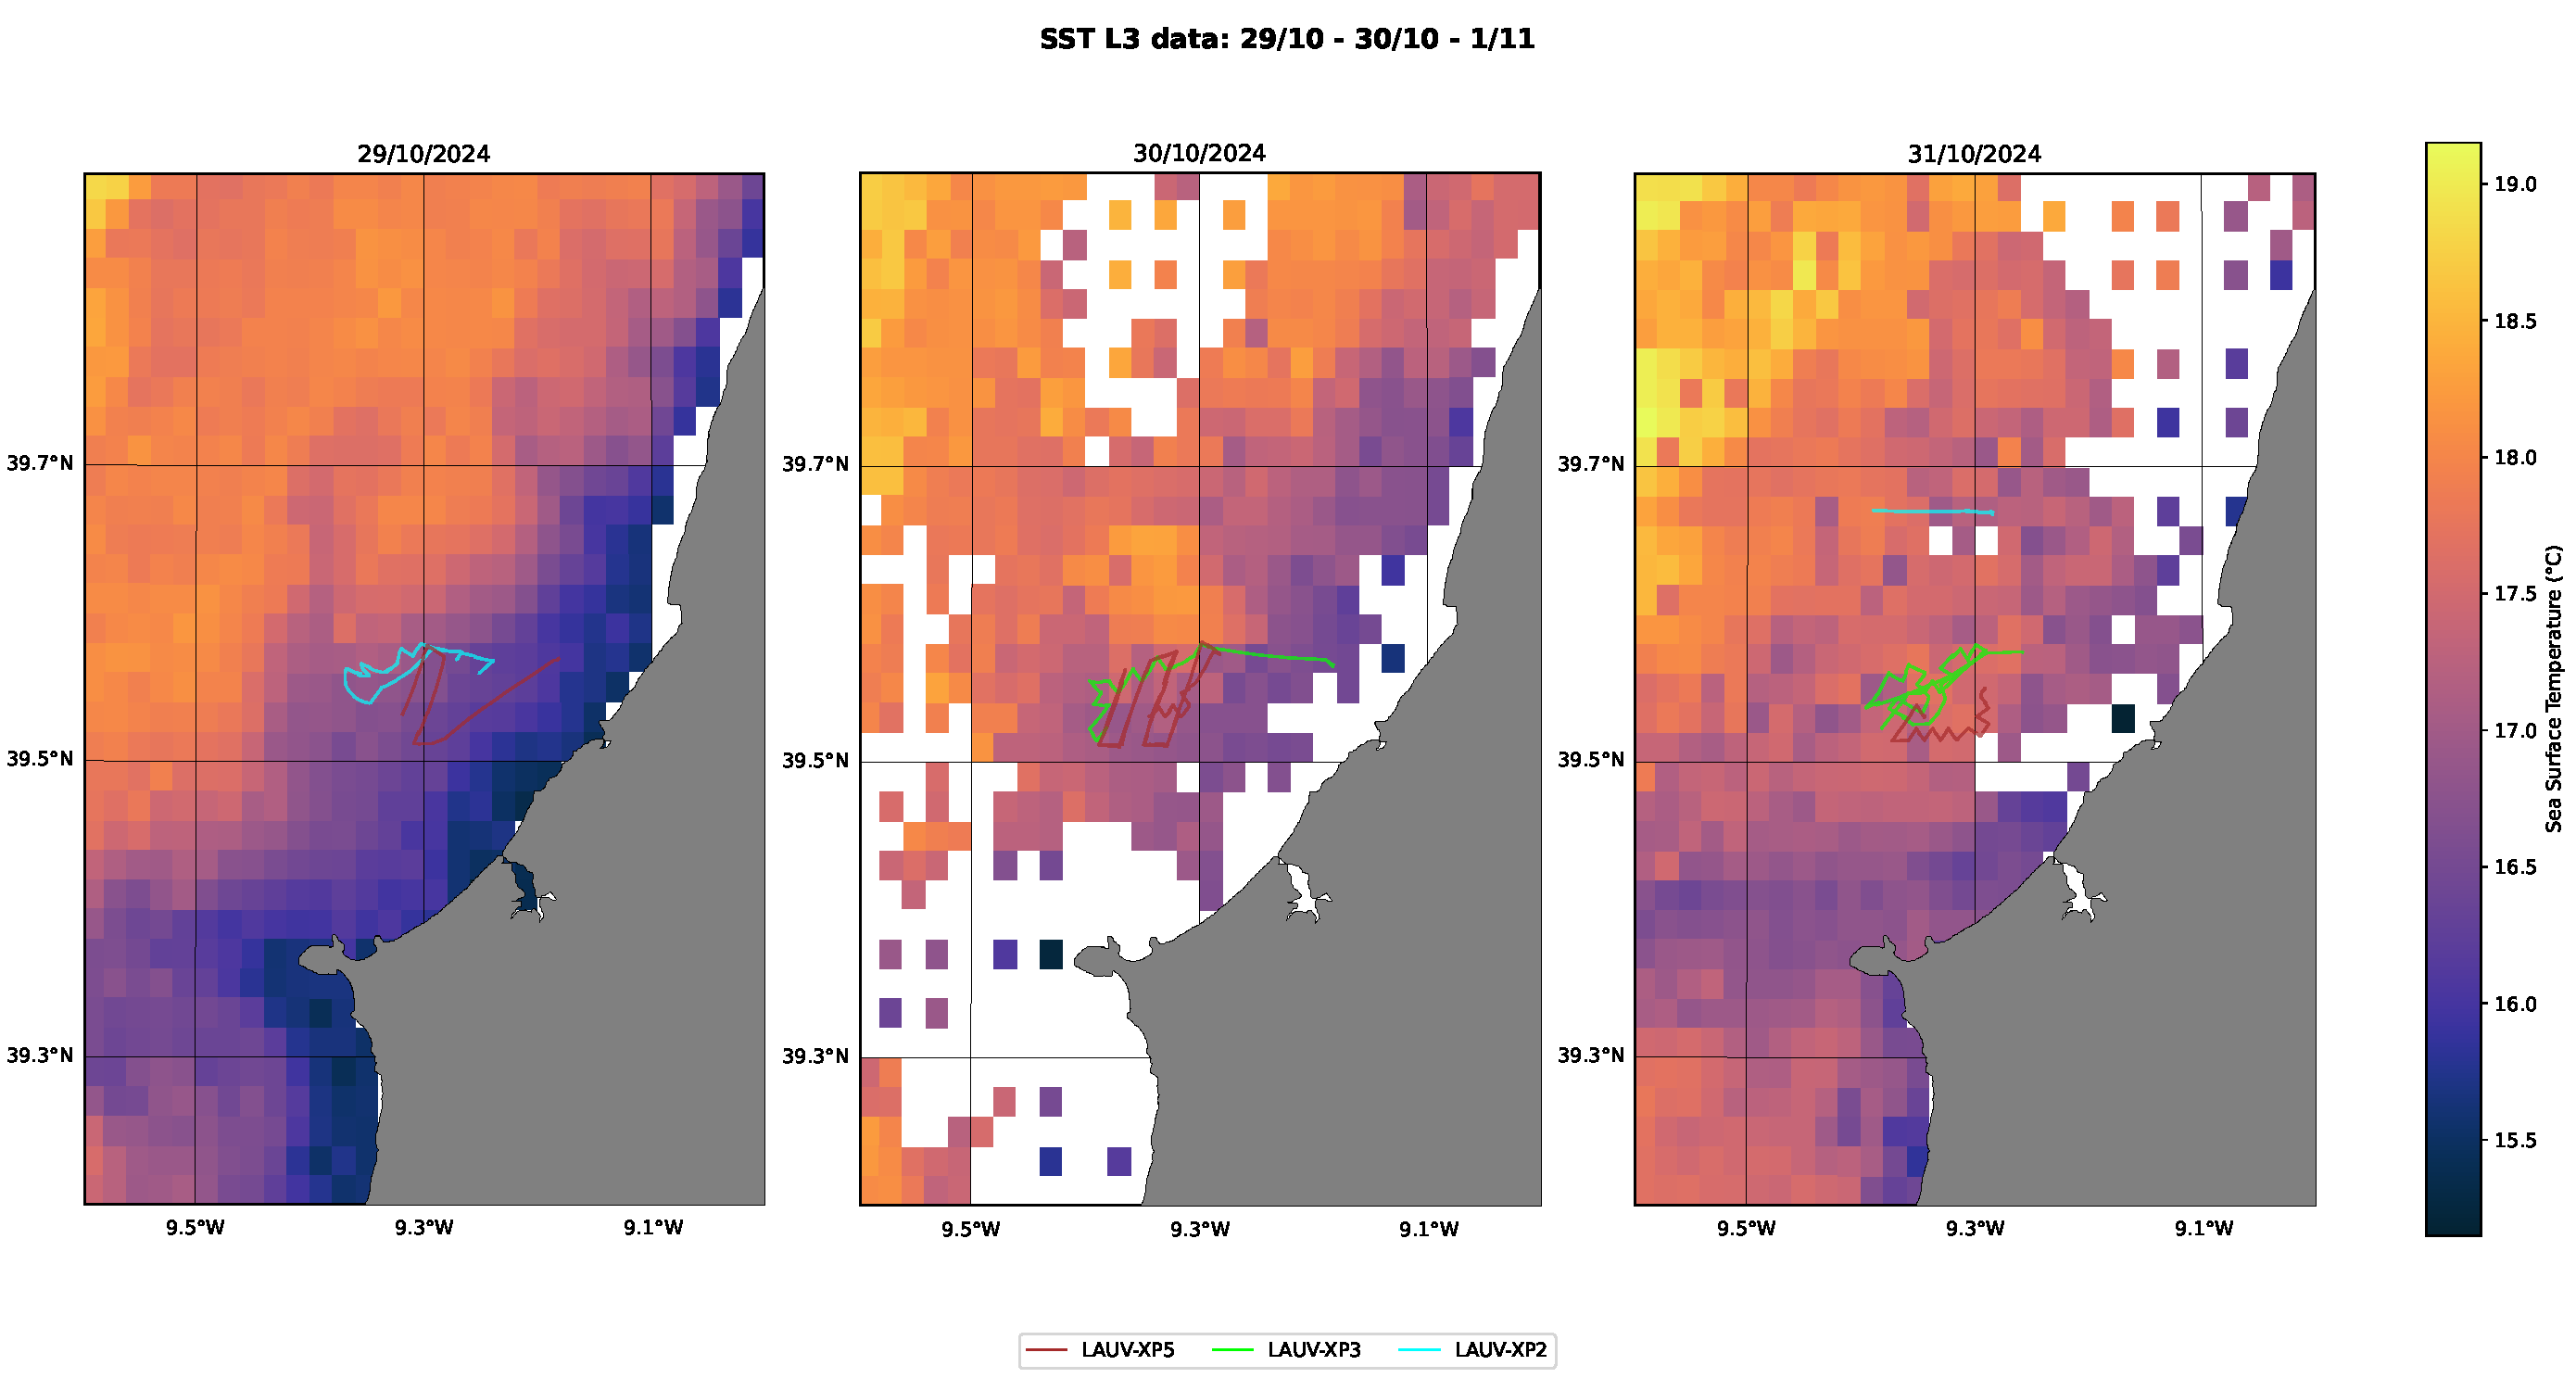
\includegraphics[width=1\linewidth]{fig/SST_L3_color1.pdf}}
  \subfigure[Temperature data collected by AUV in depth (yy) over time
  (xx)\kcomment{-- Need better captions}]{\label{fig:temperatureprofiles}\includegraphics[width=1\linewidth]{fig/Figure2_100m.pdf}}
\end{figure}

\begin{itemize}
    \item Environmental context
    \item RMS table (all cases) + rms figure (just A+D cases)
\end{itemize}

 
\textit{- Use \textbf{subheadings} to organize different experiments or analyses.}
